\documentclass[12pt,a4paper,english]{article}
\usepackage{times}
\usepackage[utf8]{inputenc}
\usepackage{babel,textcomp}
\usepackage{mathpazo}
\usepackage{mathtools}
\usepackage{amsmath,amssymb}
\usepackage{ dsfont }
\usepackage{listings}
\usepackage{graphicx}
\usepackage{ mathrsfs }
\usepackage{float}
\usepackage{subfig} 
\usepackage[colorlinks]{hyperref}
\usepackage[usenames,dvipsnames,svgnames,table]{xcolor}
\usepackage{textcomp}
\definecolor{listinggray}{gray}{0.9}
\definecolor{lbcolor}{rgb}{0.9,0.9,0.9}
\lstset{backgroundcolor=\color{lbcolor},tabsize=4,rulecolor=,language=python,basicstyle=\scriptsize,upquote=true,aboveskip={1.5\baselineskip},columns=fixed,numbers=left,showstringspaces=false,extendedchars=true,breaklines=true,
prebreak=\raisebox{0ex}[0ex][0ex]{\ensuremath{\hookleftarrow}},frame=single,showtabs=false,showspaces=false,showstringspaces=false,identifierstyle=\ttfamily,keywordstyle=\color[rgb]{0,0,1},commentstyle=\color[rgb]{0.133,0.545,0.133},stringstyle=\color[rgb]{0.627,0.126,0.941},literate={å}{{\r a}}1 {Å}{{\r A}}1 {ø}{{\o}}1}

% Use for references
\usepackage[square,comma,numbers]{natbib}
%\DeclareRobustCommand{\citeext}[1]{\citeauthor{#1}~\cite{#1}}

% Fix spacing in tables and figures
%\usepackage[belowskip=0pt,aboveskip=5pt]{caption}
%\setlength{\intextsep}{10pt plus 2pt minus 2pt}

% Change the page layout
%\usepackage[showframe]{geometry}
\usepackage{layout}
\setlength{\hoffset}{-0.5in}  % Length left
\setlength{\voffset}{-0.8in}  % Length on top
\setlength{\textwidth}{470pt}  % Width /597pt
\setlength{\textheight}{672pt}  % Height /845pt
\setlength{\footskip}{25pt}

\newcommand{\VEV}[1]{\langle#1\rangle}
\title{FYS4150 - Project 4}
\date{}
\author{ Kristoffer Langstad\\ \textit{krilangs@uio.no}}

\begin{document}%layout
\maketitle
\begin{abstract}
In this project we want to find the phase transition at a critical temperature $T_C$ for a thermodynamic system with the Ising model in 2D from a ferromagnet phase to a paramagnet phase. This is a binary system where we look at the spins (up and down) for objects that interact only with its nearest neighbor at with different lattice sizes. We will use Monte Carlo and Metropolis algorithms develop the Ising model to solve the system numerically. Properties of the system are evaluated to find the number of Monte Carlo (MC) cycles needed to reach the system equilibrium. For a simple 2x2 lattice we have analytical values that we compare our numerics with. For this case we get best results as equal results within 4 leading digits for the mean energy and mean absolute magnetic moment with $10^7$ Monte Carlo cycles and $T=1.0$, while we get equal results within 3 leading digits for the specific heat and the susceptibility. Then for the evaluation of the 20x20 lattice for $T=1.0$ and $T=2.4$ with both an ordered and random initial spin orientation of the objects, we find that the system reaches the equilibrium state after around 8000 Monte Carlo cycles per lattice (which in this case represents time). For the random initial spins, the curves of the evaluated properties are much smoother and fluctuate less than the ordered. We also see that the higher temperature have a bigger affect on the values we evaluate than the lower temperature. We also find that the number of accepted configurations as a function of the temperature in the domain $T\in[1.0, 2.4]$ increase almost as an exponential with the temperature. For the probability distribution $P(E)$, which also is the number of times a given energy appears in the MC cycles, we see that the most probable energy for $T=1.0$ is more or less the ground state with energy -800. With increased temperature $T=2.4$, we get increased entropy and most likely energy around -490$\rightarrow$ -470. So a low energy is the same as the object has a low probability of jumping to the next state. For the evaluation of the Ising model near the critical temperature $T_C$ for lattices $L=[40,60,80,100]$, temperatures $T\in[2.15, 2.35]$, stepsize $\Delta T=0.002$ and MC cycles $5\cdot10^5$ we find the numerical critical temperature $T_C=2.268$ for the specific heat and $T_C=2.292$ for susceptibility, which indicate the phase transition. With a linear regression for the critical temperatures found for the specific heat and susceptibility, we get get a critical temperature of $T_C=2.263$ for the system. The analytical critical temperature is given as $T_C\approx2.269$ (\citet{PhysRev.65.117}), which compared to the numerical is equal with 2 leading digits. The critical temperature gets closer to the analytical in the thermodynamic limit $L\rightarrow\infty$.
\end{abstract}

\section{Introduction}
\label{sect:Introduction}
To study thermodynamics we can use statistical mechanics. A very popular method to do this is the Ising model. With this model we can simulate phase transitions for a magnetic system from a quantum mechanical perspective from a ferromagnet phase to a paramagnet phase. The model can then evaluate binary states for atomic spins (up and down) in a lattice of different sizes, where the spins only interact with its nearest neighbors. The phase transitions occur at a critical temperature from a system of a finite magnetic moment to a phase with zero magnetization.

In this project we will use the two-dimensional Ising model to find the phase transitions in a magnetic system for lattices of different sizes. For the lattices we have binary values as up and down. Since we use a 2D model, we have analytical values for the critical temperature which denotes the phase transitions. First we will evaluate a 2x2 lattice by using the Ising model and Monte Carlo and Metropolis algorithms to be used as benchmark calculations. Then we expand to a 20x20 lattice for various temperature values to evaluate the equilibrium time and the probability distribution of the energies. Then we study the phase transitions of the system to find the critical temperature. The numerical calculations are done in C++ with QT Creator on a Windows computer, while the plotting are done in Python 3.7.

In the methods section we look at the theory and execution of the physical problems and the numerical algorithms we are using. For the 2x2 lattice we calculate numerically known analytical values for expressions like the expectation values for the energy $E(T)$, mean absolute magnetic moment $|M(T)|$, specific heat $C_V(T)$ and susceptibility $\chi(T)$. Then we expand to a 20x20 lattice to see when the most likely state (equilibrium time) is reached with different temperatures. After the steady state is found, we find the probability distributions for the energies to have specific values. Then we evaluate for several lattice sizes $L=[40,60,80,100]$ to find the critical temperature of the system, which indicates the phase transition. In the results section we present and discuss the results we get from the numerical calculations. These results are also compared with analytical values for the 2x2 lattice case, and the analytical value for the critical temperature by \citet{PhysRev.65.117}. In the conclusion section, we present a conclusion to the project.

\section{Methods}
\label{sect:Methods}
The theory of this project is mainly from chapter 13 in \citet{ComPhys}. The theory for the numerical algorithms are from chapter 12 in \citet{ComPhys}.
\subsection{Ising Model Theory}
\label{subsect:Ising}
To study the phase transitions in a binary magnetic system with finite temperatures, we will use the two-dimensional Ising model. In this system we look at objects with either spin up or spin down in a lattice of given sizes. The energy of this system for a state $i$ can be expressed as
\begin{equation}
\label{eq:E_ising}
E_i=-J\sum_{\langle kl\rangle}^{N}s_k s_l-\mathscr{B}\sum_{k}^{N}s_k ,
\end{equation}
with $s_k=\pm 1$, $N$ the total number of spins, $J$ is a coupling constant for strength interaction between neighboring spins, $\langle kl\rangle$ indicates a sum over the nearest neighbors only and $\mathscr{B}$ is an external magnetic field interacting with the magnetic moment set up by the spins. For this project we will assume a ferromagnetic ordering with $J>0$, and we will neglect the externally applied magnetic field ($\mathscr{B}=0$). We will also use periodic boundary conditions in this project.

We want to calculate expressions like the expectation values for the energy $\langle E\rangle$ and for the mean absolute magnetic moment (mean magnetization) $\langle |M|\rangle$, the specific heat with constant volume $C_V$ and the susceptibility $\chi$. To do this we need a probability distribution like the Boltzmann distribution in statistical mechanics as
\begin{equation}
\label{eq:Prob_dist}
P_i(\beta)=\frac{e^{-\beta E_i}}{Z},
\end{equation}
where $P_i$ is the probability of the system being in a configuration $i$, $\beta=\frac{1}{k_BT}$, $k_B$ is Boltzmann's constant, $E_i$ is the energy of a microstate $i$ and $Z$ is a partition function for canonical ensemble given as the sum over all microstates $m$
\begin{equation}
\label{eq:Part_func}
Z=\sum_{i=1}^{m}e^{-\beta E_i}.
\end{equation}
The magnetization of the system of a state $i$ can be expressed as
\begin{equation}
\label{eq:M_ising}
M_i=\sum_{k}^{N}s_k.
\end{equation}

 To calculate the expectation values we will use the Boltzmann distribution (eq. \ref{eq:Prob_dist}) and the partition function (eq. \ref{eq:Part_func}).  The expectation value of the energy is then given as:
\begin{equation}
\label{eq:exp_E}
\langle E(T)\rangle=\sum_{i=1}^{m}E_iP_i(T)=\frac{1}{Z}\sum_{i=1}^{m}E_ie^{-\beta E_i}
\end{equation}

The expectation value of the absolute magnetization is given as:
\begin{equation}
\label{eq:exp_M}
\langle |M(T)|\rangle=\sum_{i=1}^{m}|M_i|P_i(T)=\frac{1}{Z}\sum_{i=1}^{m}|M_i|e^{-\beta E_i}
\end{equation}
We use the absolute value of the magnetization since just using the expectation value of the magnetization will always be zero. This comes from that we can always find an equal number of states with equal magnetization with opposite sign. 

The specific heat of the system is given as the derivative of the expectation value of the energy with respect to the temperature $T$:
\begin{equation}
\label{eq:exp_CV}
C_V(T)=\frac{\partial}{\partial T}\langle E(T)\rangle=\frac{1}{k_BT^2}\left(\langle E^2(T)\rangle-\langle E(T)\rangle^2\right)=\frac{\sigma_E^2}{k_BT^2}
\end{equation}
So the specific heat can be related to the variance of the energy $\sigma_E^2$.

The susceptibility of the system can be expressed as $\beta$ times the derivative of the expectation value of the absolute magnetization with respect to $\beta$ as:
\begin{equation}
\label{eq:exp_susc}
\chi(T)=\beta\frac{\partial}{\partial \beta}\langle |M(T)|\rangle=\beta\left(\langle |M(T)|^2\rangle-\langle |M(T)|\rangle^2\right)=\beta \sigma_M^2
\end{equation}
So the susceptibility can be related to the variance of the magnetization $\sigma_M^2$.

\subsection{Analytic Expressions}
\label{subsect:analytic}
First we look at a 2x2 lattice ($L=2$), which contains four object. We will study $\langle E(T)\rangle$ (eq. \ref{eq:exp_E}), $\langle |M(T)|\rangle$ (eq. \ref{eq:exp_M}), $C_V(T)$ (eq. \ref{eq:exp_CV}) and $\chi(T)$ (eq. \ref{eq:exp_susc}) as functions of the temperature $T$ scaled as $[T]=k_BT/J$. We will also have $[k_B]=\frac{energy}{temperature}$ and $[J]=energy$. By scaling the rest of the expectation values accordingly, we get; the energy scaled as $[E]=J$, the magnetization scaled as $[|M|]=1$, the specific heat scaled as $[C_V]=\frac{J^2}{k_BT^2}$ and the susceptibility scaled as $[\chi]=\frac{1}{k_BT}$.

For the 2x2 lattice with either spin up or spin down, the total number of possible microstates is $2^4=16$. Since this is a very simple case, we can calculate analytical values for the partition function and the four expectation values already mentioned. By using the equations for energy (\ref{eq:E_ising}) and magnetization (\ref{eq:M_ising}) we get the values in Table \ref{tab:analytic}.

\begin{table}[htbp]
	\centering
	%\hspace{-1cm}
	\begin{tabular}{ |c|c|c|c| }
		\hline \rule{0pt}{13pt}
		\# $\uparrow$ & $g$ & $E[J]$ & $M$ \\
		\hline \rule{0pt}{13pt}
		4 & 1 & -8 & 4 \\
		\hline \rule{0pt}{13pt}
		3 & 4 & 0 & 2  \\
		\hline \rule{0pt}{13pt}
		2 & 4 & 0 & 0 \\
		\hline \rule{0pt}{13pt}
		2 & 2 & 8 & 0 \\
		\hline \rule{0pt}{13pt}
		1 & 4 & 0 & -2 \\
		\hline \rule{0pt}{13pt}
		0 & 1 & -8 & -4 \\
		\hline 
	\end{tabular}	
	\caption{Table for the number of microstates for the 2x2 lattice, where the total number of microstates is 16 for the four object. To the left we have the number of up spins. Then we have $g$ (degeneracy or \# of configurations), which is the number of times this microstate can occur. Then we have the energy and magnetization for the microstates.}
	\label{tab:analytic}
\end{table}
From the values in Table \ref{tab:analytic}, we first derive the partition function:
\begin{align}
\label{eq:Z_analytic}
Z=\sum_{i=1}^{m=16}e^{-\beta E_i}=12+2e^{-8\beta J}+2e^{8\beta J}
\end{align}
The expectation expression for the energy is:
\begin{align}
\label{eq:E_analytic}
\langle E\rangle=\frac{1}{Z}\sum_{i=1}^{m=16}E_ie^{-\beta E_i}=\frac{16J}{Z}\left(e^{-8\beta J}-e^{8\beta J}\right)
\end{align}
The expectation expression for the mean magnetization is:
\begin{align}
\label{eq:M_analytic}
\langle |M|\rangle=\frac{1}{Z}\sum_{i=1}^{m=16}|M_i|e^{-\beta E_i}=\frac{8}{Z}\left(2+e^{8\beta J}
\right)
\end{align}
The expectation expression for the specific heat is:
\begin{align}
\label{eq:CV_analytic}
C_V=\frac{1}{k_BT^2}\left(\langle E^2(T)\rangle-\langle E(T)\rangle^2\right)=\frac{128J^2}{k_BT^2Z^2}\left(8+12e^{-8\beta J}+12e^{8\beta J}\right)
\end{align}
The expectation expression for the susceptibility is:
\begin{align}
\label{eq:Xi_analytic}
\chi=\beta\left(\langle |M(T)|^2\rangle-\langle |M(T)|\rangle^2\right)=\frac{32\beta}{Z}\left((1+e^{8\beta J})-\frac{2}{Z}(2+e^{8\beta J})^2\right)
\end{align}

We will for the rest of the project use natural units such that $k_B=1$ and also use $J=1$. To test the 2x2 lattice, we implement the Ising model with Metropolis algorithm (explained in the Numerical Algorithms section \ref{subsect:Algo}) to calculate the analytical expectation values numerically for a temperature $T=1.0$ $ [k_BT/J]$, and test for different numbers of Monte Carlo cycles up to $10^8$ to see when we achieve a good agreement with the analytical values.

\subsection{Numerical Algorithms}
\label{subsect:Algo}
The coding was done on a Windows 10 computer with 8GB RAM. The Python code for plotting was run in Python 3.7, while the C++ codes for doing the main calculations were done and run in Qt Creator as mentioned in the \textit{README.md} at the GitHub repository \ref{sect:appendix}. The codes can be found in the Code-folder at the same GitHub repository.
\subsubsection{Markov Chains}
\label{subsubsect:Markov}
The Markov chains does a selected probability for making a move. The new move does not depend on the previous history of the algorithm, only on the last step. The Markov chain is used several time in Monte Carlo simulations to make new states, which are random. After many runs with an initial random state for Markov chains, the solutions goes towards a most likely state or an equilibrium state for the system in thermodynamics. The Markov chain equation is defined as
\[w_i(t+\epsilon)=\sum_{j}W(j\rightarrow i)w_j(t).\]
This reaches the equilibrium state when $t\rightarrow\infty$ where there is no time dependence (optimally). In the equation above for the Markov chain, $w_i$ is the time dependent PDF normalized of a state $i$ and $W$ goes as the normalized probability of jumping from a state $j$ to a state $i$ and is time-independent. The transition probability $W$ is in most cases unknown, so we rewrite it as the product of two probabilities as
\[W(j\rightarrow i)=T(j\rightarrow i)A(j\rightarrow i).\]
$T(j\rightarrow i)$ is the likelihood for having a transition from state $j$ to state $i$. This is as for the Ising model we are using in this project, which is a likelihood for picking a specific spin $\sim \frac{1}{N}$. $A(j\rightarrow i)$ is the likelihood for accepting the suggested move in $T$. Assuming $T$ and $A$ time-independent, the time PDF can then be rewritten to 
\[w_i(t+\epsilon=1)=\sum_{j}\left[T(j\rightarrow i)A(j\rightarrow i)w_j(t)+w_i(t)T(i\rightarrow j)(1-A(i\rightarrow j))\right].\]
Since the probabilities are normalized ($\epsilon=1$)we can further rewrite the time PDF:
\[w_i(t+1)-w_i(t)=\sum_{j}\left[T(j\rightarrow i)A(j\rightarrow i)w_j(t)-w_i(t)T(i\rightarrow j)A(i\rightarrow j)\right]\]
For $t\rightarrow\infty$ we get $w_i(t)\rightarrow w_i$ and $w_i(t+1)\rightarrow w_i$ as mentioned earlier. This again leads to \[w_i(t+1)-w_i(t)=0,\] and  
\[w_jT(j\rightarrow i)A(j\rightarrow i)=w_iT(i\rightarrow j)A(i\rightarrow j).\]
This now leads to what is called detailed balance to avoid cyclic solutions:
\begin{equation}
\label{eq:balance}
\frac{w_i}{w_j}=\frac{T(j\rightarrow i)A(j\rightarrow i)}{T(i\rightarrow j)A(i\rightarrow j)}
\end{equation}

\subsubsection{Metropolis}
\label{subsubsect:Metro}
For solving the Ising model we will use the Metropolis algorithm. This uses Markov chain processes when doing the calculations. We are using the Boltzmann distribution in equation \ref{eq:Prob_dist} as our PDF, such that we end up with:
\[w_i=\frac{1}{Z}e^{-\beta E_i}\quad \bigwedge\quad w_j=\frac{1}{Z}e^{-\beta E_j}\]
Inserting these into the detailed balance (eq. \ref{eq:balance}) yields:
\begin{align*}
\frac{e^{-\beta E_i}}{e^{-\beta E_j}}=\frac{T(j\rightarrow i)A(j\rightarrow i)}{T(i\rightarrow j)A(i\rightarrow j)}
\end{align*}
For the simplest Metropolis algorithm (brute force Metropolis) we assume symmetric transition probability $T(j\rightarrow i)=T(i\rightarrow j)$ \cite{ComPhys}. From the new detailed balance with this assumption, we get:
\begin{equation}
\label{eq:Brute_Metro}
\frac{A(j\rightarrow i)}{A(i\rightarrow j)}=\frac{e^{-\beta E_i}}{e^{-\beta E_j}}=e^{-\beta(E_i-E_j)}=e^{-\beta\Delta E}
\end{equation}
By looking at this equation we can see that the most probable energy is the lowest. This alone would not lead to anything useful, since it would always move to the lowest energy in the system. This would lead to biased statistical averages \footnote{Chapter 12.5: The Metropolis Algorithm and Detailed Balance \cite{ComPhys}}. We want our Markov processes to being able to reach every possible state of the system given enough time and any random starting point. To fix this problem we set the acceptance probability $A$ as:
\[A(j\rightarrow i)=\begin{cases} e^{-\beta \Delta E},\quad &\Delta E>0\\
\quad 1,\quad &\text{else}
\end{cases}\]
This says that a move to a lower energy state is always accepted with value 1. For a move to a higher energy state, then we must check this acceptance probability. 

A thing to notice is that since we, in any lattice, will only consider affections from the nearest neighbors for the energies of the objects, we can do some simplifications to the numerical calculation algorithms. We are limited to five number of energy changes as $[-8J,-4J, 0, 4J, 8J]$. This means that for given $T$ values, we can precalculate all the probabilities $e^{-\beta \Delta E}$, saving a lot of CPU time.

For the Ising model in 2D, we will have $2N$ number of configurations where $N=L\times L$ is the number of spins for a lattice of length $L$ \footnote{\label{note2}Chapter 13.5: The Metropolis Algorithm and the Two-dimensional Ising Model \cite{ComPhys}}. The Metropolis is the algorithm to use since it only calculates ratios between probabilities and neglects the partition function. The following Metropolis algorithm is from \citet{ComPhys}$^{\ref{note2}}$:
\begin{enumerate}
	\item Create an initial state with initial energy $E_{init}$ with either a fixed spin configuration or a random spin configuration in the lattice.
	\item Choose a random object in the lattice and change the configuration by flipping the spin of that object only. Then compute the new energy of this trial state $E_t$.
	\item Calculate $\Delta E=E_t-E_{init}$.
	\item If $\Delta E\leq0$, we accept the new configuration, and go to step 7.
	\item If $\Delta E>0$, we calculate $w=e^{-\beta \Delta E}$.
	\item Compare the calculated probability $w$ to a random number $r\in[0,1]$. If $r\leq w$, we accept the new configuration, else we keep the old configuration.
	\item Update the various expectation values.
	\item Repeat steps 2-7 for the number of Monte Carlo cycles for each sweep through the lattice, to obtain a sufficiently good representation of states.
	\item Divide the expectation values by the total number of MC cycles.
\end{enumerate}

\subsection{Equilibrium State}
\label{subsect:Equilibrium}
Next we want to find when the system reaches the most likely state for a 20x20 lattice. We will use the number of Monte Carlo cycles per sweeps of the lattice as time. We want the equilibrium time of the system to being able to calculate the expectation values in a stable system. Before the most likely state, the system is not stable. To study at which this time this occurs, we will look at the expectation values of the energy and magnetization for $T=1.0$ and $T=2.4$ to study the temperature dependency of the system for $2\cdot10^4$ MC cycles. We will also use both an ordered and a random spin orientation as starting configuration. From these analysis we should reach a conclusion for how many Monte Carlo cycles are needed for the system to reach the most likely state/equilibrium state. For further analysis, we also plot the total number of accepted configurations as function of both the number of Monte Carlo cycles and the temperature separately.

\subsection{Probability Distribution}
\label{subsect:Prob_dist}
For the same lattice with $L=20$ and temperatures $T=1.0$ and $T=2.4$, we calculate the probability distribution of the energy, $P(E)$, by counting the number of times a given energy appears in the Monte Carlo cycles for $4\cdot10^4$ number of Monte Carlo cycles. With the time/number of MC cycles needed to reach the equilibrium state, we choose to start calculating the probability distribution after this point in time (around 9000 MC cycles), which is when the system is more stable. We also calculate the variance \[\sigma_E^2=\langle E^2(T)\rangle-\langle E(T)\rangle^2\] and the standard deviation $\sigma_E$ in the energy.

\subsection{Phase Transitions}
\label{subsect:Phase_trans}
Near a critical temperature $T_C$, the behavior of the system starts to change by a power law behavior. The mean magnetization is now given by
\begin{equation}
\label{eq:mag_TC}
\langle M(T)\rangle\sim(T-T_C)^{\beta},
\end{equation}
where $\beta=1/8$ is the critical exponent. This relation is also applied to the specific heat and susceptibility
\begin{align}
\label{eq:CV_TC}
C_V(T)&\sim |T_C-T|^{\alpha}\\
\label{eq:Xi_TC}
\chi(T)&\sim |T_C-T|^{\gamma},
\end{align}
where $\alpha=0$ and $\gamma=7/4$. A $T\rightarrow T_C$, the spins become more and more correlated. This gives that the correlation length increases closer to the critical temperature. The correlation length is expected to be of the order of the lattice spacing for $T>>T_C$. The divergent behavior of the correlation length near $T_C$ is 
\begin{equation}
\label{eq:corr_len}
\xi(T)\sim |T_C-T|^{-\nu}.
\end{equation}
With the correlation length spanning the whole system characterizes a second-order phase transition. $\xi$ will always be proportional with the size of the lattice, since we are restricted to a finite lattice. By using finite size scaling relations we can relate the behavior at finite lattices with the results for an infinitely large lattice. The critical temperature scales as
\begin{equation}
\label{eq:TC_scale}
T_C(L)-T_C(L=\infty)=aL^{-\frac{1}{\nu}},
\end{equation}
where $a$ is a constant and $\nu$ is the same as in \ref{eq:corr_len}. At the critical temperature $T=T_C$, we obtain new expressions for the mean magnetization
\begin{equation}
\label{eq:crit_M}
\langle M(T)\rangle\sim(T-T_C)^{\beta}\rightarrow L^{-\frac{\beta}{\nu}},
\end{equation}
the specific heat 
\begin{equation}
\label{eq:crit_CV}
C_V(T)\sim |T_C-T|^{-\gamma}\rightarrow L^{\frac{\alpha}{\nu}},
\end{equation}
and the susceptibility
\begin{equation}
\label{eq:crit_xi}
\chi(T)\sim |T_C-T|^{-\alpha}\rightarrow L^{\frac{\gamma}{\nu}}.
\end{equation}

To study the phase transition behavior of the Ising model for our system close to the critical temperature, we will look at the Ising model as a function of lattice sizes $L\times L$. We will do this by calculating all the expectation values for the energy, magnetization, specific heat and susceptibility again as functions of the temperature for $L=[40,60,80,100]$, $T\in[2.15, 2.35]$, temperature stepsize $\Delta T=0.002$ and $5\cdot10^5$ number of MC cycles. We will then plot these results to try to find and indication of a phase transition. 

With these results we will use equation \ref{eq:TC_scale} for the critical temperature with $\nu=1$, to estimate $T_C$ in the thermodynamic limit $L\rightarrow \infty$ for the same lattices as for the phase transition. For $a$ we will use different lattices and subtract to find
\begin{equation}
\label{eq:find_a}
a=\frac{T_C(L_i)-T_C(L_j)}{L_i^{-1}-L_j^{-1}}.
\end{equation}
This critical temperature above is what we want to find. This is done by using that the critical temperature is when the specific heat and susceptibility has their maximum for each lattice. So we will use that the critical temperature seems to evolve linearly to perform a linear regression after finding the critical temperatures for each lattice separately for $C_V$ and $\chi$, and use this as an approximation to the systems critical temperature. This numerically calculated critical temperature we use to compare to an analytically found value found by \citet{PhysRev.65.117}, which is found to be
\begin{equation}
\label{eq:TC_analytic}
\frac{k_BT}{J}=\frac{2}{\ln(1+\sqrt{2})}\approx 2.269.
\end{equation}

\section{Results}
In the Data folder at the GitHub repository (\ref{sect:appendix}) we have text-files containing all the produced data to be evaluated either in tables or as plots. The corresponding plots can be found in the Figures folder.

For the first case with a $2x2$ lattice and with temperature $T=1.0 k_BT/J$ we calculated the expectation values numerically to compare with analytical values (calculated in section \ref{subsect:analytic}) as seen in Table \ref{tab:lattice_2} for some chosen number of Monte Carlo cycles. In the text file \textit{Lattice\_2x2} in the Data-folder at the GitHub repository \ref{sect:appendix} we see more values. In the mentioned table we see that our numerical values are within three leading digits after $10^6$ number of MC cycles for the energy and magnetization. For the specific heat and susceptibility we need $10^7$ MC cycles to get the same accuracy. For $10^8$ we see that the values start to get worse for some reason. 

\begin{table}[htbp]
	\centering
	%\hspace{-1cm}
	\begin{tabular}{ |c|c|c|c|c| }
		\hline \rule{0pt}{13pt}
		 & Analytical & MC=$10^6$ & MC=$10^7$ & MC=$10^8$\\
		\hline \rule{0pt}{13pt}
		$\langle E(T)\rangle [J]$ & -7.9839283 & -7.9837760 & -7.9839400 & -7.9841136 \\
		\hline \rule{0pt}{13pt}
		$\langle |M(T)|\rangle [1]$ & 3.9946429 & 3.9947200 & 3.9946598 & 3.9947162 \\
		\hline \rule{0pt}{13pt}
		$C_V(T)[\frac{J^2}{k_BT^2}]$ & 0.12832933 & 0.12952878 & 0.12823488 & 0.12684906 \\
		\hline \rule{0pt}{13pt}
		$\chi(T) [\frac{1}{k_BT}]$ & 0.016042958 & 0.015428122 & 0.015953482 & 0.015789361 \\
		\hline 
	\end{tabular}	
	\caption{Table for the mean energy $E$, mean absolute magnetic moment $|M|$, specific heat $C_V$ and susceptibility $\chi$ for both analytical and numerical values for a $2x2$ lattice and $T=1.0 k_BT/J$. Here we see that after $10^6$ Monte Carlo cycles, the numerical values get quite close to the analytical values. We get the best values for $10^7$ MC cycles, since with $10^8$ cycles the values start to get worse again.}
	\label{tab:lattice_2}
\end{table}

Then we wanted to find when the most likely state was reached. To do this we used a $20x20$ lattice for $T=1.0$ and $T=2.4$. We also calculated for a case with ordered initial spin orientation, and for a case with random initial spin orientation. We evaluated the expectation values for the energy, magnetization and the total number of accepted configurations as functions of the number of MC cycles (sweeps per lattice) representing time. For the number of accepted configurations, we also plotted it as function of the temperature. 

In Figure \ref{fig:equil_E} we have three plots of the expectation values for the energy for ordered (fig. \ref{fig:Ordered_E1} and \ref{fig:Ordered_E2}) and random (fig. \ref{fig:Random_E}) initial spin orientation for $T=1.0$ and $T=2.4$. From these plots we see that the expectation energies are higher for the higher temperature. This makes sense since increasing the temperature also increases the entropy of the system, which then increases the energy of the system. By comparing the ordered and random initial spins, we see that the random spins reaches the equilibrium state much earlier than for ordered spin. For the random spin the energy values also decrease with number of MC cycles, while for ordered spin the energies increase with number of MC cycles. For the lower temperature the system also seems to reach the equilibrium state a little earlier than for the higher temperature.

\begin{figure}[htbp]
	%\hspace*{-2.5cm}
	\subfloat[Expectation values for the energy with ordered initial spin orientation and $T=1.0$. Here it looks like the system reaches an equilibrium state after around 7000 MC cycles. The energies are also very close to the ground state energy. \label{fig:Ordered_E1} ]{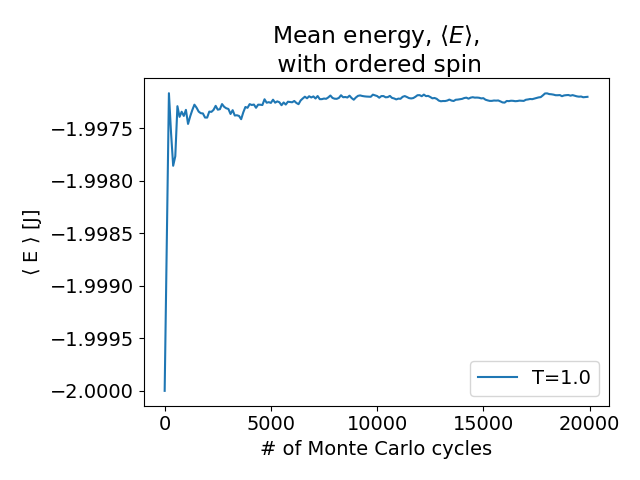
\includegraphics[width=0.5\linewidth]{E_Ordered_1.png}}
	\hspace{0.5em}
	\subfloat[Expectation values for the energy with ordered initial spin orientation and $T=2.4$. Here it looks like the system reaches an equilibrium state after around 8000 MC cycles. In this case the energies are much higher than for the lower $T$ since the entropy of the system has increased with the increased $T$ value. \label{fig:Ordered_E2} ]{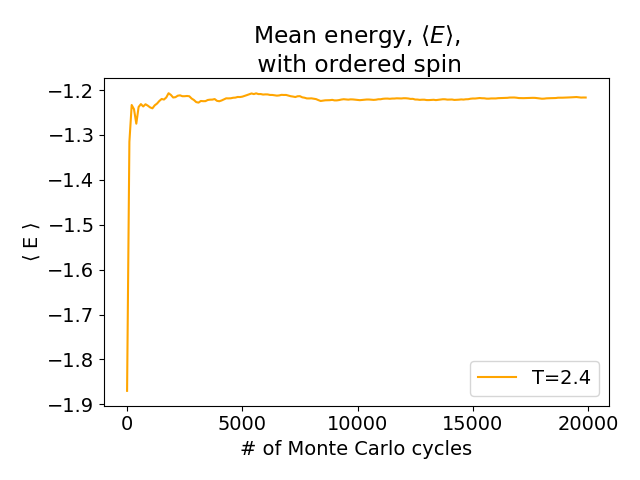
\includegraphics[width=0.5\linewidth]{E_Ordered_2_4.png}}\\
	\subfloat[Expectation values for the energy with random initial spin orientation and both temperatures. Here it looks like the system reaches an equilibrium state after around 4000 MC cycles for $T=1.0$. For $T=2.4$ it looks like the system reach equilibrium around 5000 MC cycles. \label{fig:Random_E}]{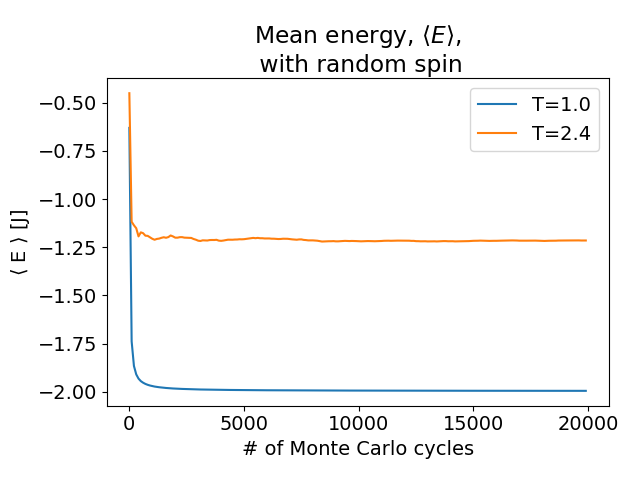
\includegraphics[width=0.6\linewidth]{E_Random.png}}
	\caption{Here we have plots for the expectation values for the energy splitted into one for ordered initial spin orientation and $T=1.0$, one for ordered initial spin orientation and $T=2.4$ and one for random initial spin orientation for both temperatures. Here we see that with random initial spin the system reaches the equilibrium state much earlier than for the ordered spin. The energies for higher $T$ value are much higher than for lower $T$.\label{fig:equil_E}}
\end{figure}

In Figure \ref{fig:equil_M} we have three plots of the expectation values for the absolute magnetization for ordered (fig. \ref{fig:Ordered_M1} and \ref{fig:Ordered_M2}) and random (fig. \ref{fig:Random_M}) initial spin orientation for $T=1.0$ and $T=2.4$. From Figure \ref{fig:Ordered_M1} we see that the magnetization values does not change much and reaches equilibrium state around 7000 MC cycles. From Figure \ref{fig:Ordered_M2} we see that the values drops much more before reaching the equilibrium state around 8000 MC cycles. For the random spins in Figure \ref{fig:Random_M} the curve for lower $T$ reaches equilibrium state much earlier at around 4000MC cycles, while for higher $T$ it reaches equilibrium state around 8000 MC cycles. These expectation figures behaves like the opposite as the energies in Figure \ref{fig:equil_E}. So when the expectations energy of the system increases, the expectation values of the magnetization decreases. We also see that for lower temperature, the system seem to be more stable since it reaches the equilibrium state earlier. From these two figures we can conclude that the system reaches the equilibrium state earliest around 8000 MC cycles, so to be safe we can say that the equilibrium state has been reached after 9000 MC cycles.

\begin{figure}[htbp]
	%\hspace*{-2.5cm}
	\subfloat[Expectation values for the absolute magnetization with ordered initial spin orientation and $T=1.0$. Here it looks like the system reaches an equilibrium state after around 7000 MC cycles. The magnetization values changes very little. \label{fig:Ordered_M1} ]{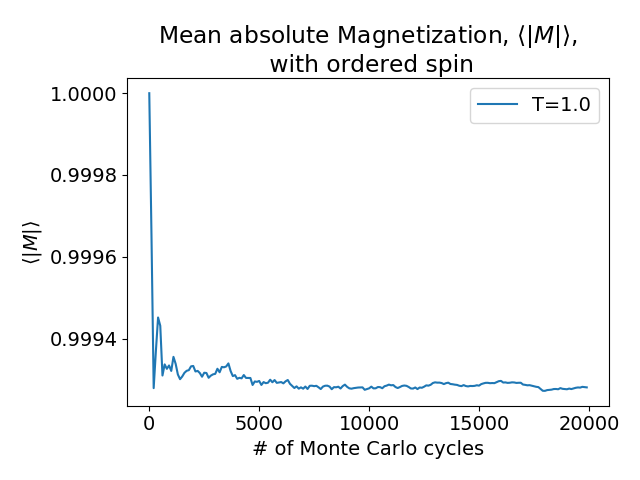
\includegraphics[width=0.5\linewidth]{M_Ordered_1.png}}
	\hspace{0.5em}
	\subfloat[Expectation values for the absolute magnetization with ordered initial spin orientation and $T=2.4$. Here it looks like the system reaches an equilibrium state after around 8000 MC cycles. In this case the magnetization values are much lower than for the lower $T$. \label{fig:Ordered_M2} ]{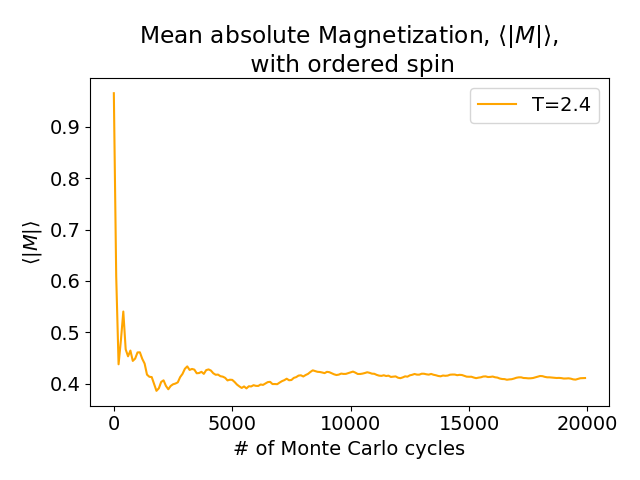
\includegraphics[width=0.5\linewidth]{M_Ordered_2_4.png}}\\
	\subfloat[Expectation values for the absolute magnetization with random initial spin orientation and both temperatures. Here it looks like the system reaches an equilibrium state after around 4000 MC cycles for $T=1.0$. For $T=2.4$ it looks like the system reach equilibrium around 8000 MC cycles. \label{fig:Random_M}]{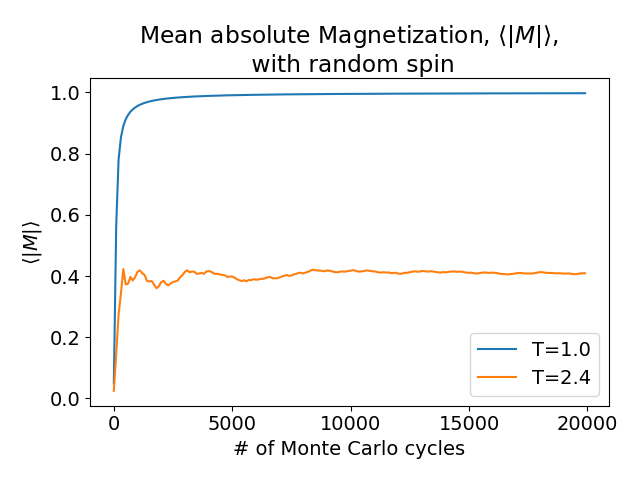
\includegraphics[width=0.6\linewidth]{M_Random.png}}
	\caption{Here we have plots for the expectation values for the absolute magnetization splitted into one for ordered initial spin orientation and $T=1.0$, one for ordered initial spin orientation and $T=2.4$ and one for random initial spin orientation for both temperatures. Here we see that with random initial spin the system reaches the equilibrium state much earlier than for the ordered spin. The energies for higher $T$ value are much higher than for lower $T$.\label{fig:equil_M}}
\end{figure}

In Figure \ref{fig:equil_Nconfigs} we have three plots for the total number of accepted configurations for ordered (fig. \ref{fig:Ordered_Nconfigs1} and \ref{fig:Ordered_Nconfigs2}) and random (fig. \ref{fig:Random_Nconfigs}) initial spin orientation for $T=1.0$ and $T=2.4$. These figures behave the same way like the expected energy of the system. So there is a connection between the energy and the number of accepted configurations. This also applies to the temperature of the system, where the number of accepted configurations increase much more for higher temperature for ordered initial spins. For the random initial spin the total number of configurations decrease much more for lower temperature, and seem to be much more stable than the rest. In Figure \ref{fig:acceptvsT} we see the temperature dependence on the total number of accepted configurations. The number of accepted configurations increases close to an exponential as the temperature increases.

\begin{figure}[htbp]
	%\hspace*{-2.5cm}
	\subfloat[Total number of accepted configurations normalized as function of the number of MC cycles with ordered initial spin orientation and $T=1.0$. The number of accepted config values changes very little, and is very low. \label{fig:Ordered_Nconfigs1} ]{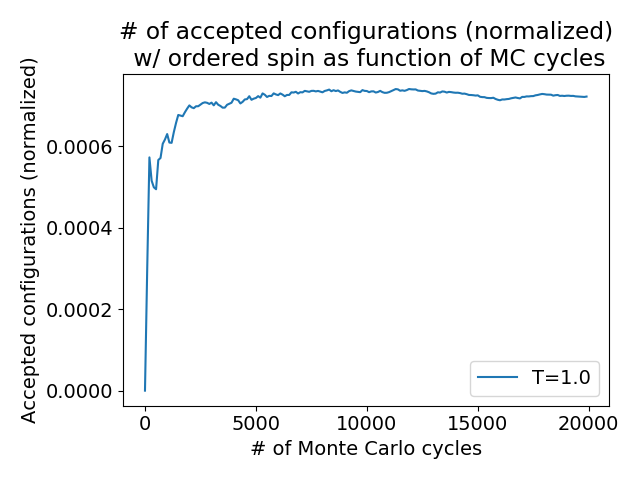
\includegraphics[width=0.5\linewidth]{Accpt_Ordered_1.png}}
	\hspace{0.5em}
	\subfloat[Total number of accepted configurations normalized as function of the number of MC cycles with ordered initial spin orientation and $T=2.4$. In this case the number of accepted configs are much higher than for the lower $T$. \label{fig:Ordered_Nconfigs2} ]{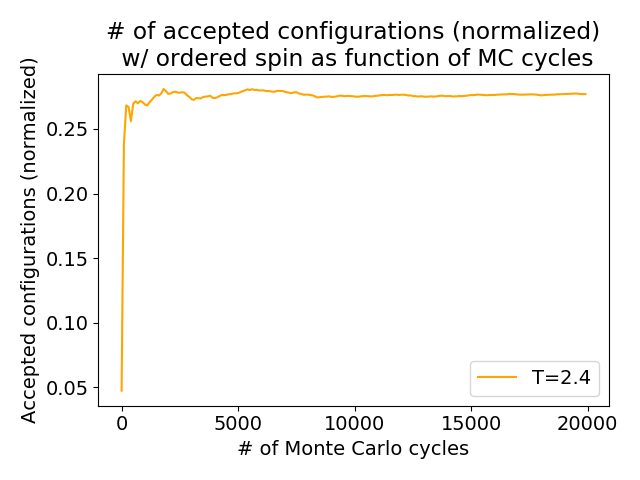
\includegraphics[width=0.5\linewidth]{Accpt_Ordered_2_4.png}}\\
	\subfloat[Total number of accepted configurations normalized as function of the number of MC cycles with random initial spin orientation and both temperatures. \label{fig:Random_Nconfigs}]{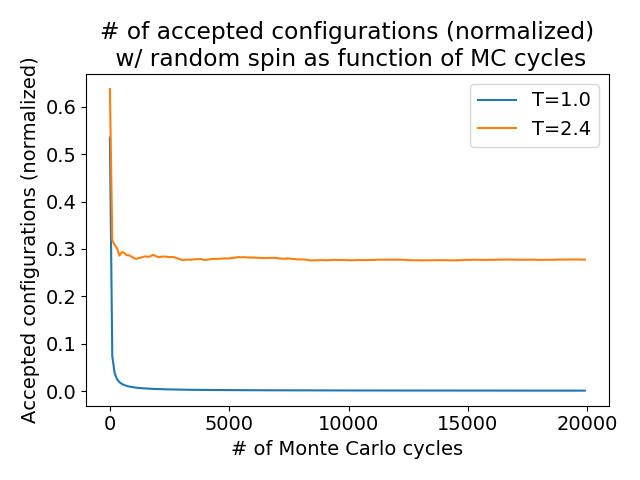
\includegraphics[width=0.6\linewidth]{Accpt_Random.png}}
	\caption{Here we have plots for the total number of accepted configurations normalized as function of the number of MC cycles splitted into one for ordered initial spin orientation and $T=1.0$, one for ordered initial spin orientation and $T=2.4$ and one for random initial spin orientation for both temperatures. Here we see that with random initial spin the system reaches the equilibrium state much earlier than for the ordered spin. The number of accepted configurations are much higher for higher $T$. The curves behave like for the energy curves in Figure \ref{fig:equil_E}. So there is a connections between the expected energy of the system and the number of accepted configurations.\label{fig:equil_Nconfigs}}
\end{figure}

\begin{figure}[htbp]
	\centering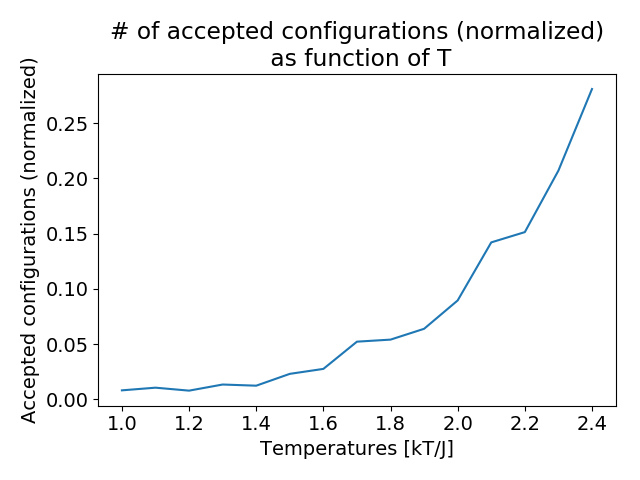
\includegraphics[width=0.5\linewidth]{AccptVsT.png}
	\caption{Figure for the number of accepted configurations normalized as function of the temperature. Here we see that the number of accepted configurations increase almost exponentially as the temperature increase. \label{fig:acceptvsT}}
\end{figure}

For the probability distribution $P(E)$ for the $L=20$ lattice and $4\cdot10^4$ MC cycles, we counted the number of times a given energy appears in the MC cycles for $T=1.0$ (fig. \ref{fig:Prob1}) and $T=2.4$ (fig. \ref{fig:Prob2}). Since we found that the system reach the equilibrium state after around 9000 MC cycles, we start to count the probability distribution after this. For the low temperature $T=1.0$ the most probable energy is the ground state energy -800. This means that the probability of an object in the system to jump to the next state is very low. For the higher temperature $T=2.4$, the most probable energy is around -470 to -490, which are the two spikes on each side of the middle. Since this resembles a Gaussian we could expect that the real most probable energy would be between these two spikes. This probability has a standard deviation of $\sigma_E=3.04$ and variance $\sigma_E^2=9.27$. So now the probability of an object to jump to the next state is much higher since the entropy of the system is higher.. This probability distribution is similar to a Gaussian distribution. This distribution has a higher standard deviation of $\sigma_E=56.62$ and variance $\sigma_E^2=3206$.

\begin{figure}[htbp]
	%\hspace*{-2.5cm}
	\subfloat[Probability distribution for $T=1.0$ as function of the energy. Here almost all the counted energies are the ground state energy at -800. So the most probable energy of the system is the ground state energy. This means that there is a low probability of the object to jump to the next state. \label{fig:Prob1} ]{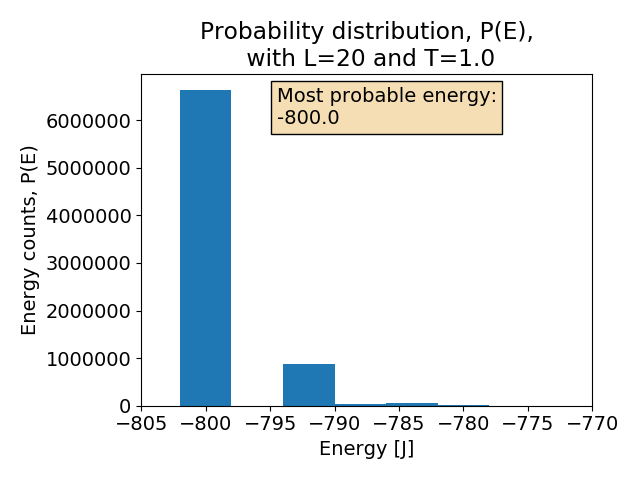
\includegraphics[width=0.5\linewidth]{Prob_1.png}}
	\hspace{0.5em}
	\subfloat[Probability distribution for $T=2.4$ as function of the energy. Here the energies are more distributed around the most probable energy of around -470. The curve looks like a Gaussian. The given most probable energy in the figure is the highest number of counted energy. \label{fig:Prob2} ]{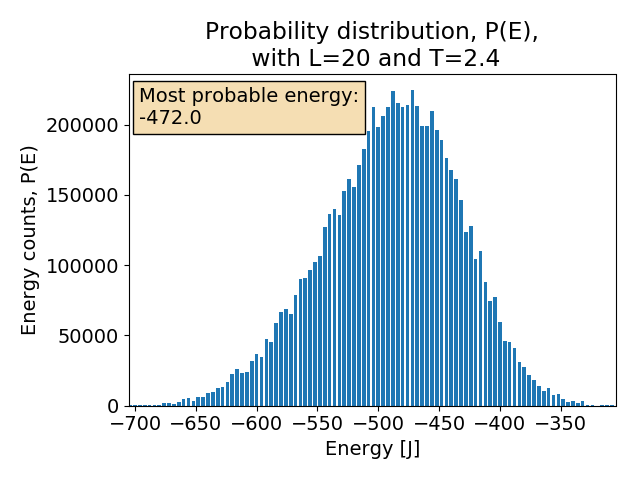
\includegraphics[width=0.5\linewidth]{Prob_2_4.png}}
	\caption{Figures for the probability distributions $P(E)$ as the number of times a given energy appears in the MC cycles fro $T=1.0$ (fig. \ref{fig:Prob1}) and $T=2.4$ (fig. \ref{fig:Prob2}).\label{fig:prob_dist}}
\end{figure}

To study the phase transition of the system with the two-dimensional Ising model near the critical temperature $T_C$, we calculated the expectation values for $\langle E(T)\rangle$ (fig. \ref{fig:Phase_E}) and $\langle |M(T)|\rangle$ (fig. \ref{fig:Phase_M}), the specific heat $C_V(T)$ (fig. \ref{fig:Phase_CV}) and the susceptibility $\chi(T)$ (fig. \ref{fig:Phase_Xi}) for lattices $L=[40,60,80,100]$, temperatures $T\in[2.15,2.35]$, $\Delta T=0.002$ and $5\cdot10^5$ MC cycles. The phase transition plots can be seen in Figure \ref{fig:Phases}. In the phase plot for the magnetization, we see that as $L\rightarrow\infty$ the corresponding curves converges. This convergence point is the critical temperature which from \citet{PhysRev.65.117} is given as an analytical value as $T_C\approx2.269$. The phase transition is where the critical temperature is. This is also indicated where the specific heat and susceptibility has their maximum \cite{ComPhys}\footnote{Chapter 13.4: Phase Transitions and Critical Phenomena}. The phase before the transition is the ferromagnetic phase, while the phase after is the paramagnetic phase. In the paramagnetic phase we see that the magnetization drops towards zero. For the energy we see that in the paramagnetic phase, the energy increases more and more as $L\rightarrow\infty$. For the specific heat and the susceptibility, the curves gets a higher and higher maximum peak as $L\rightarrow\infty$.

\begin{figure}[htbp]
	%\hspace*{-2.5cm}
	\subfloat[Phase plot for the expectation values for the energy $\langle E(T)\rangle$. \label{fig:Phase_E} ]{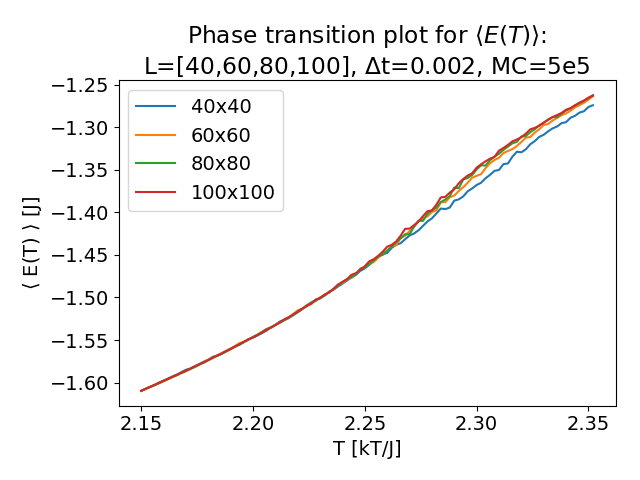
\includegraphics[width=0.5\linewidth]{Phase_E(T).png}}
	\hspace{0.5em}
	\subfloat[Phase plot for the expectation values for the absolute magnetization $\langle |M(T)|\rangle$. \label{fig:Phase_M} ]{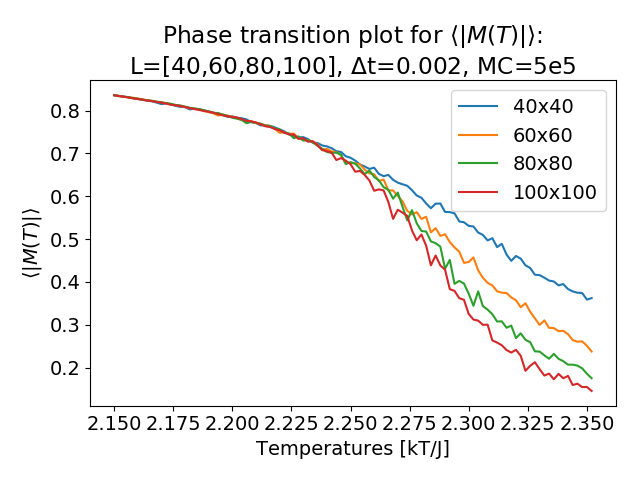
\includegraphics[width=0.5\linewidth]{Phase_M(T).png}}\\
	\subfloat[Phase plot for the specific heat $C_V(T)$. \label{fig:Phase_CV}]{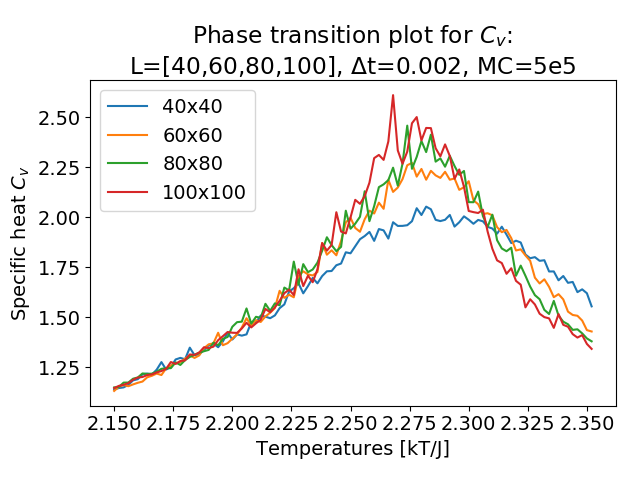
\includegraphics[width=0.5\linewidth]{Phase_Cv(T).png}}
	\hspace{0.5em}
	\subfloat[Phase plot for the susceptibility $\chi(T)$. \label{fig:Phase_Xi}]{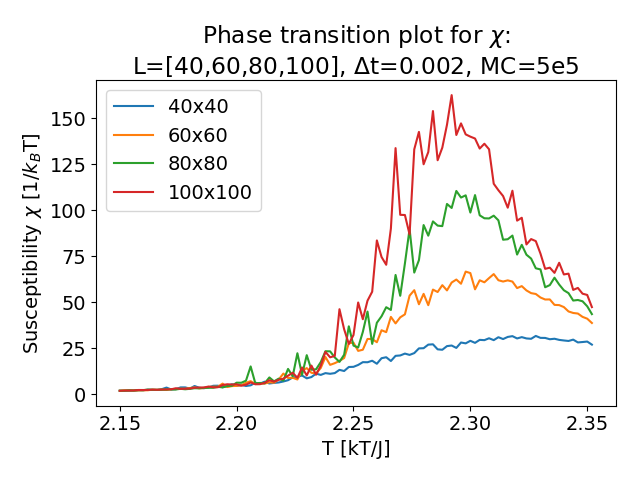
\includegraphics[width=0.5\linewidth]{Phase_Xi(T).png}}
	\caption{Here we see phase plots for the expectation values of the energy and absolute magnetization, the specific heat and the susceptibility for lattices $L=[40,60,80,100]$, temperatures $T\in[2.15,2.35]$, $\Delta T=0.002$ and $5\cdot10^5$ MC cycles near the critical temperature $T_C$. The phase transition is indicated where the specific heat and susceptibility has their maximum, called the critical point (ch. 13.4 in \citet{ComPhys}).\label{fig:Phases}}
\end{figure}

In Figure \ref{fig:TC} we see the phase transition plot for the specific heat again, but now we have plotted the critical temperatures for each lattice and the analytic critical temperature by \citet{PhysRev.65.117} ($T_C\approx2.269$). In Table \ref{tab:TC} we see the critical temperatures for the lattices and the analytical $T_C$. As $L\rightarrow\infty$ we see that the critical temperatures converges to the analytical $T_C$, where $T_C=2.268$ for the specific heat is very close to the analytical. The critical temperature for the susceptibility $T_C=2.292$ is further away from the analytical. By taking the mean of linear regressions for the critical temperature for the specific heat and the susceptibility, we get an estimation for the critical temperature of the system as $T_C\approx2.263$.

\begin{table}[htbp]
	\centering
	%\hspace{-1cm}
	\begin{tabular}{ |c|c|c| }
		\hline \rule{0pt}{13pt}
		Lattice & $T_C: C_V$ & $T_C: \chi$ \\
		\hline \rule{0pt}{13pt}
		$40x40$ & 2.282 & 2.328\\
		\hline \rule{0pt}{13pt}
		$60x60$ & 2.276 & 2.298\\
		\hline \rule{0pt}{13pt}
		$80x80$ & 2.274 & 2.294\\
		\hline \rule{0pt}{13pt}
		$100x100$ & 2.268 & 2.292\\
		\hline \rule{0pt}{13pt}
		- & - & - \\
		\hline \rule{0pt}{13pt}
		Analytic: & $k_BT_C/J\approx$ & 2.269 \\
		\hline 
	\end{tabular}	
	\caption{Table for the calculated critical temperatures for the lattices for the specific heat and susceptibility of the system. As $L\rightarrow\infty$ we see that the calculated critical temperature converges to the analytic.}
	\label{tab:TC}
\end{table}

\begin{figure}[htbp]
	\centering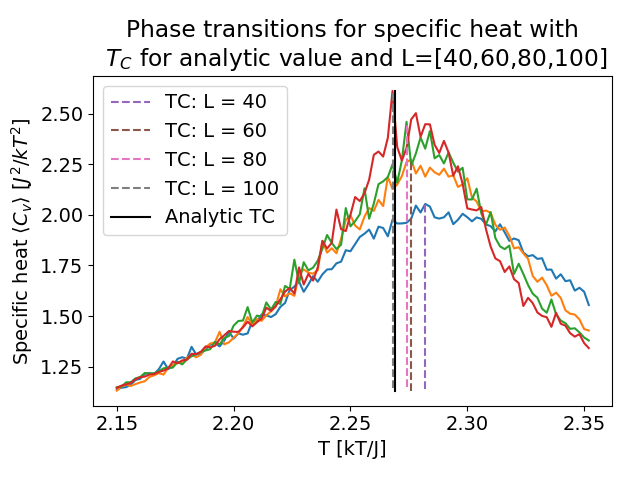
\includegraphics[width=0.8\linewidth]{CV_TC.png}
	\caption{Figure for the specific heat where the dotted straight lines indicate the individual critical temperatures for the lattices, while the black straight line indicates the analytic critical temperature from \citet{PhysRev.65.117}. We see that as $L\rightarrow\infty$, the lattice critical temperature converges towards the analytic critical temperature. \label{fig:TC}}
\end{figure}

\section{Conclusion}
In this project we have simulated a phase transition for a binary magnetic system by using the Ising model in 2D for a ferromagnetic phase to a paramagnetic phase with zero magnetization. We have used Monte Carlo and Metropolis algorithms with the Ising model to simulate the phase transition for different sizes of lattices for objects with either spin up or down.

We have calculated expectation values for a 2x2 lattice which we have compared with analytic values. For $10^7$ MC cycles we got equal results with at least three leading digits for all the expectation values we calculated. For the next case with a 20x20 lattice with both ordered and random initial spin orientation, we found that the system reaches a equilibrium state after around 9000 MC cycles. This threshold was then used as a mark to start calculating the probability distribution $P(E)$, where we ran with $4\cdot10^4$ MC cycles, by counting the number of times a given energy appeared in the MC cycles. For the lower temperature we got that the most probable energy is the ground state energy, such that an object hos a very low chance of not being in the ground state. For higher temperature, the probability of jumping states increases. For an increase in the temperature of the system, this lead to an increase in the energy and in the number of accepted configurations. This also lead to the magnetization going towards zero, as wanted. For the phase transition and critical temperature, we tested for lattice sizes $L\rightarrow\infty$ for $L=[40,60,80,100]$. Here we found the critical temperature by looking at the maximum of the specific heat for the lattices. To do this we needed enough MC cycles to get enough data. So for $5\cdot10^5$ MC cycles, $\Delta T=0.002$, $T\in[2.15,2.35]$ and $L=100$ (ideally want $L\rightarrow\infty$), we got a critical temperature $T_C=2.268$ for the specific heat and $T_C=2.292$ for the susceptibility. With the mean of the linear regressions of the found critical temperatures we get $T_C=2.263$ for the system. This is close to the analytical $T_C\approx2.269$ found by \citet{PhysRev.65.117}. In this limit at $T_C$, the system goes from a ferromagnetic phase to a paramagnetic phase.

For even better results we could be to run for larger lattice $L$ sizes, use smaller $\Delta T$ values and/or even more MC cycles. The most efficient would probably be to use more MC cycles to produce more data. By looking at the phase transition plots in Figure \ref{fig:Phases}, we see that the curves are not optimal since they are not smooth. This comes from that we have not used enough MC cycles, but they are good enough as seen when comparing the critical temperatures. The CPU time for running $5\cdot10^5$ MC cycles was around 16,5 hours. So to increase the MC cycles more, would increase the CPU time by a lot. This could be done with more time. The reason for this long time, is that the code was not properly parallelized. For some reason, the armadillo library and openMP library made an error on the used Windows computer. This error came when implementing the compiler flag \textit{-fopenmp}. Without the mentioned compiler flag, the parallelization would not be initialized. With the flag, then some of the armadillo functions would not work properly. With more time, this error could most likely have been fixed. So by parallelizing the code, the CPU time would go down drastically.

\appendix
\section{Appendix}
\label{sect:appendix}
Link to GitHub repository:\\
\url{https://github.com/krilangs/FYS4150/tree/master/Project4}

\bibliographystyle{plainnat}
\bibliography{myrefs}
\end{document}